\part{Data Prediction}
\section{Prediction of values about the data}

Some basic and general goals were defined before starting this phase, with the idea of "doing more if it's possible". Basically the main purpose was the one of, after the previous analysis, predict some values and evaluate the quality of the results.
This prediction system was not defined with some specific requirements, so the first main problem was to find a reliable, accurated and user-friendly way to predict and display prediction of values.

Since the current dataset can be considered like a time series, in this phase we will develop the data prediction system using an ARIMA machine implemented in python.

The ARIMA machine can be configured with several configurations, it allows you to have more accurated results; so the first thing was to find the right configuration of the ARIMA machine of each single input which we are interested to forecast.

During this phase of the work have been implemented 3 different subsystems for different purposes:
\begin{enumerate}
\item Evaluating System
\item Training System
\item Future Prediction System
\end{enumerate}

\newpage
\subsection{Evaluating System}
\textbf{Goal:}\\ 
Used for evaluate different configurations of ARIMA machine. \\ 
It tests 112 different configurations for each single input that we would like to forecast and report the results with each MAPE (Mean Average Percentage Error) values.

\textbf{Requirements:}\\
There are not strict requirements needed. There are no type of restriction neither about the length or about the type of data.

\textbf{Code implementation:}\\
The most important part of the code about the Evaluating System is the following.\\
Basically the method ARIMA() allows to train a model based on historic values (history) and a specific order (p,d,q). After that it's possible to call the method forecast() through the trained model and having some predictions like result.
\begin{lstlisting}
model = ARIMA(history, order=arima_order)
model_fit = model.fit(disp=0)
yhat = model_fit.forecast()[0]
\end{lstlisting}

This system will provide 112 different ARIMA configurations results for each single input, and in particular it will display the best ARIMA configuration, that is the one with the lower MAPE.

\textbf{Results:}\\
The system will display the MAPE between real value and predicted values for each single tested ARIMA machine, in particular the configuration that gives the best result.
All these results have been reported in a document and then also displayed with a 3D graphic that allows to see the MAPE value for each different order in input.



\begin{figure}[H]
	\raggedleft
	\makebox[\textwidth][c]{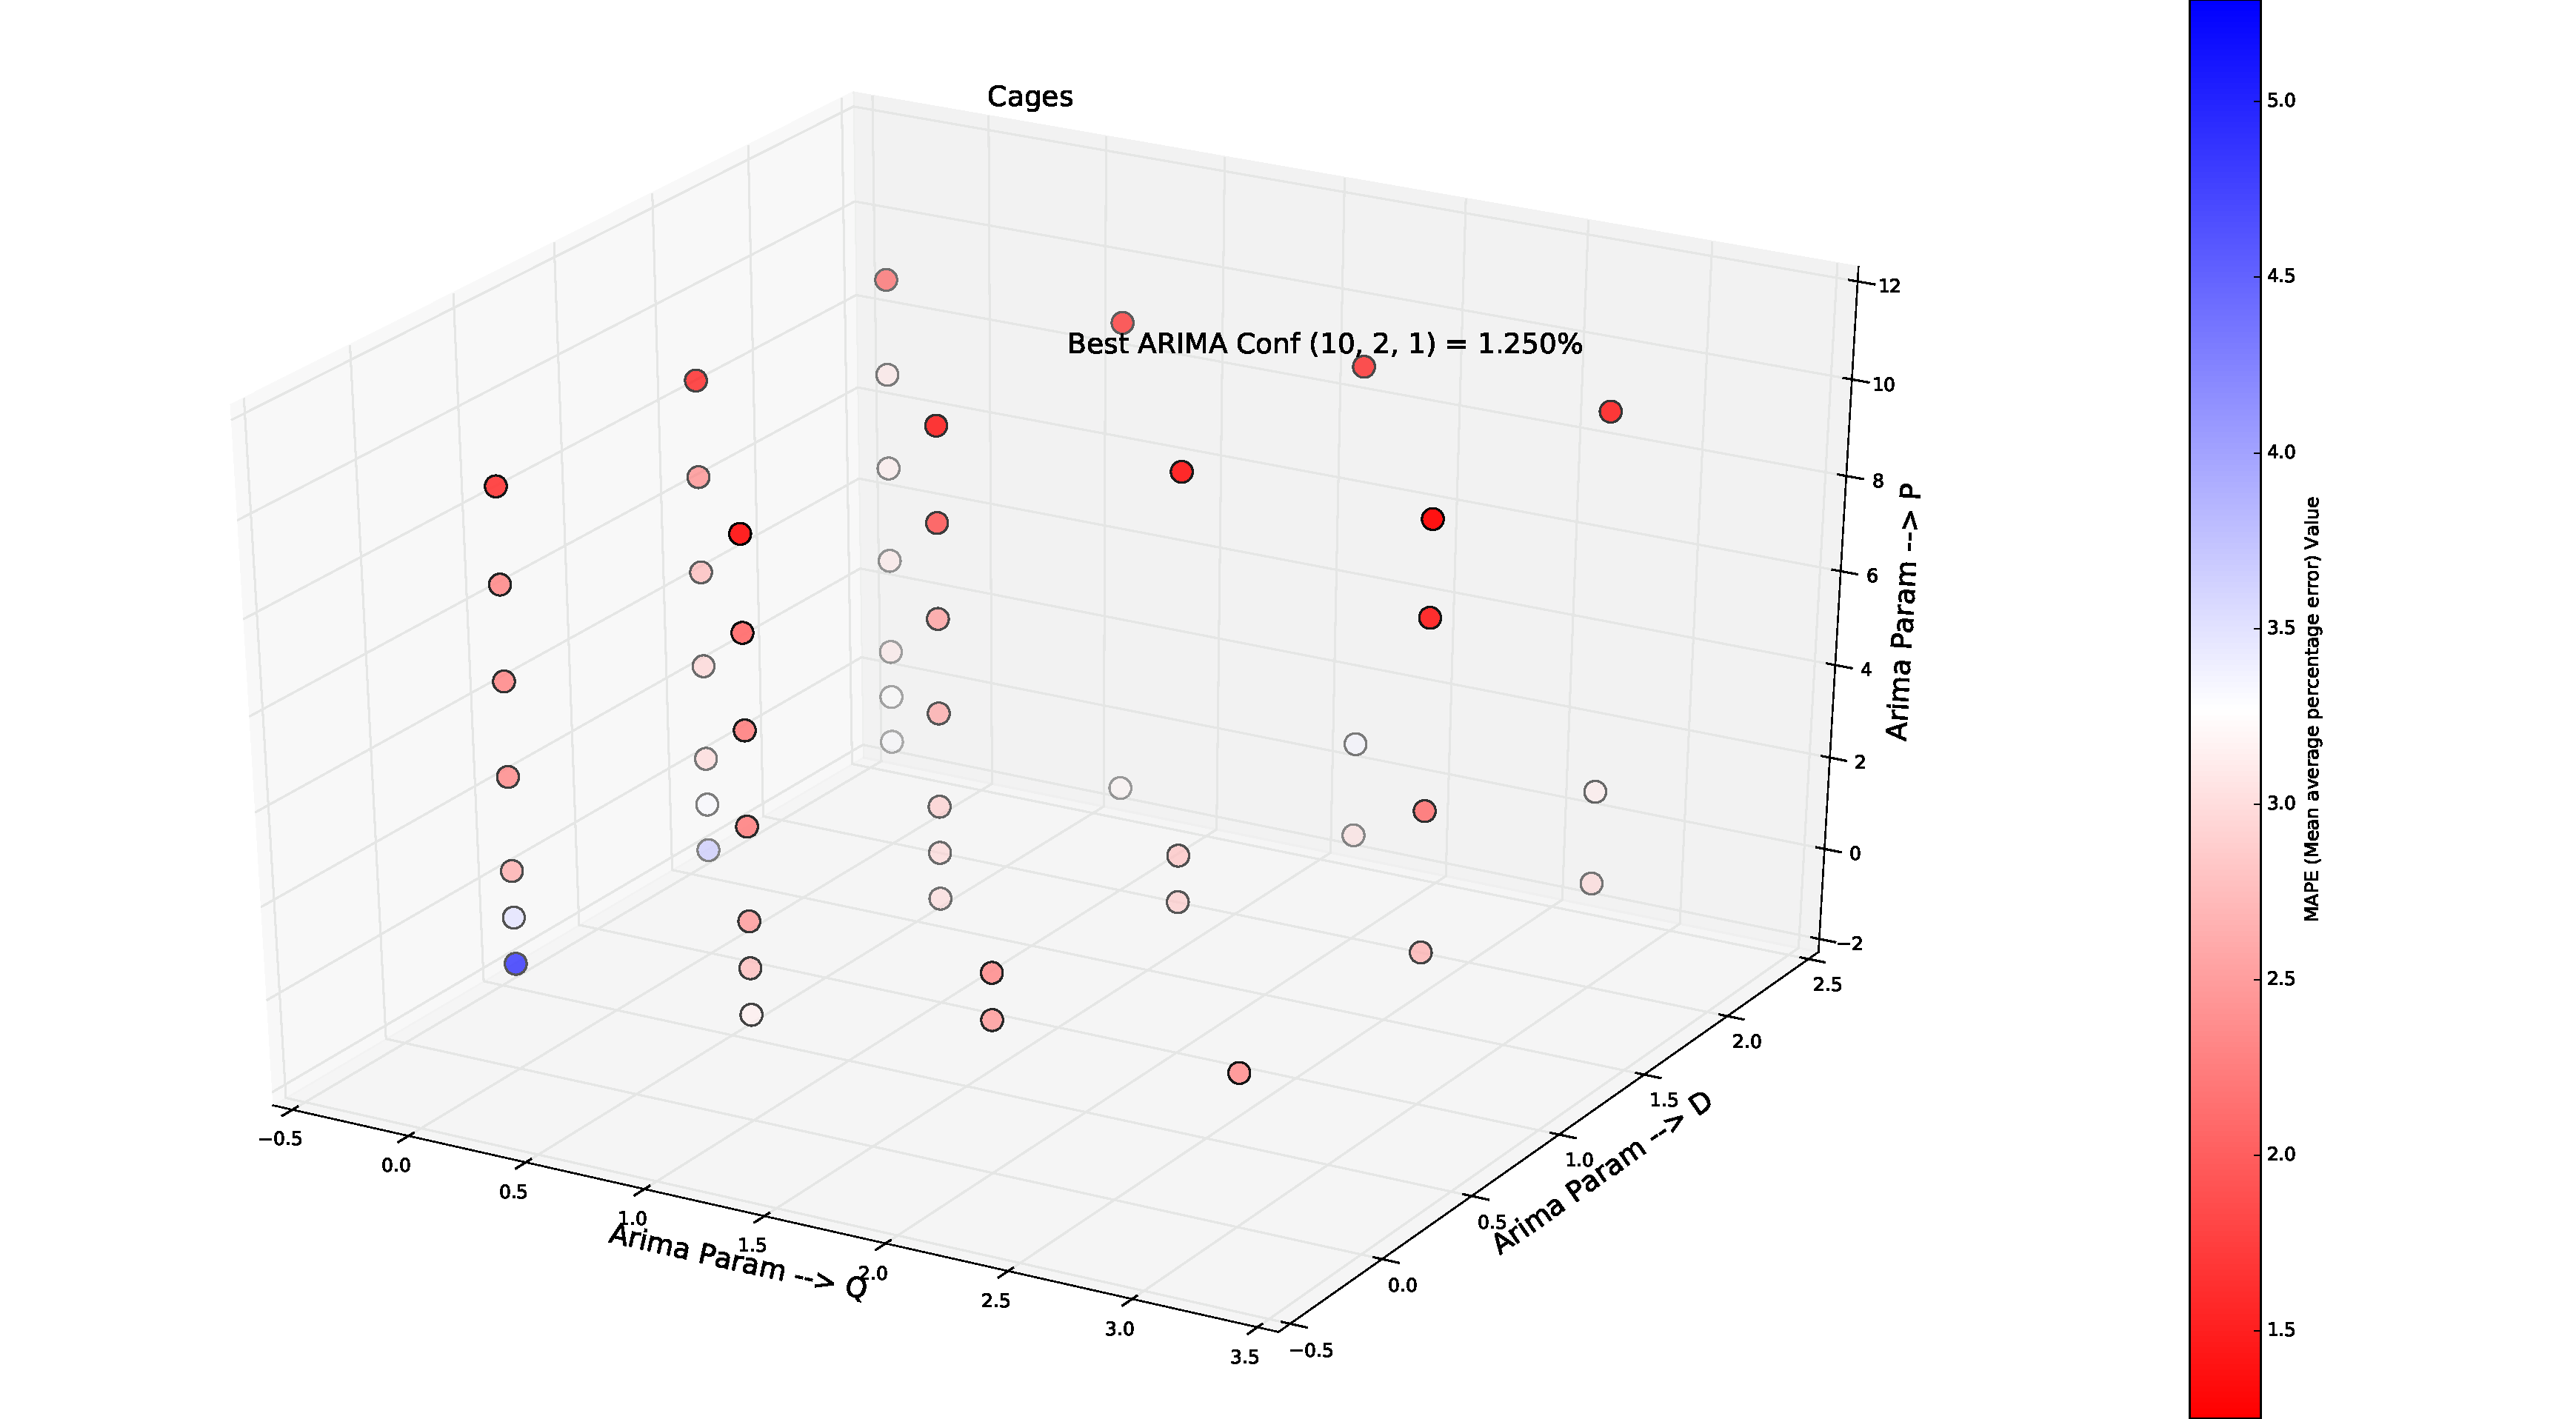
\includegraphics[width=0.7\textwidth]{Files/Cages_MAPE.pdf}}
    \caption{Graphic that displays different MAPE values for each ARIMA order.}
\end{figure}

 
 
\newpage
\subsection{Training System}
\textbf{Goal:}\\ 
This system has the goal of training/testing a specific ARIMA configuration on a particular data input, and see how much accurate it is. 

\textbf{Requirements:}\\
Since this Traning System has been used mainly for train and test the current dataset, it need to have like input a dataset that follows the same format:\\
- Data content: 144 values, 1 value for each month from 2005 to 2016

\textbf{Code implementation:}\\
First of all this system it's going to split the input data in two part:\\
- Train data: values which the ARIMA model is going to use for training. \\
- Test data: values which are hided by the forecasting model. \\
Once the ARIMA model has been created, the system will try to predict the future values, that are actually the "Test data".\\

\begin{lstlisting}
model = ARIMA(history, order=arima_order)
model_fit = model.fit(disp=0)
yhat = model_fit.forecast()[0]
\end{lstlisting}

Once the predictions have been calculated it's possible to display the "Test data" (that are the real values) and the predicted values, just to see how much the ARIMA configuration is accurate.

\begin{lstlisting}
series = pd.read_csv("Dataset.csv", usecols=[sys.argv[1]])
series.plot(color="blue", linewidth=1.5,
		 label="Series: "+sys.argv[1])


output = Series.from_csv('Output_Files/predictions.csv')
output.plot(color="red", linewidth=1.5,
		label="Prediction test:")
\end{lstlisting}

\newpage

\textbf{Results:}\\
The following picture is an output example of this training system. \\
It actually allows to have an idea about how accurate is that ARIMA configuration for predictions.
\begin{figure}[H]
	\centering
    \makebox[\textwidth][c]{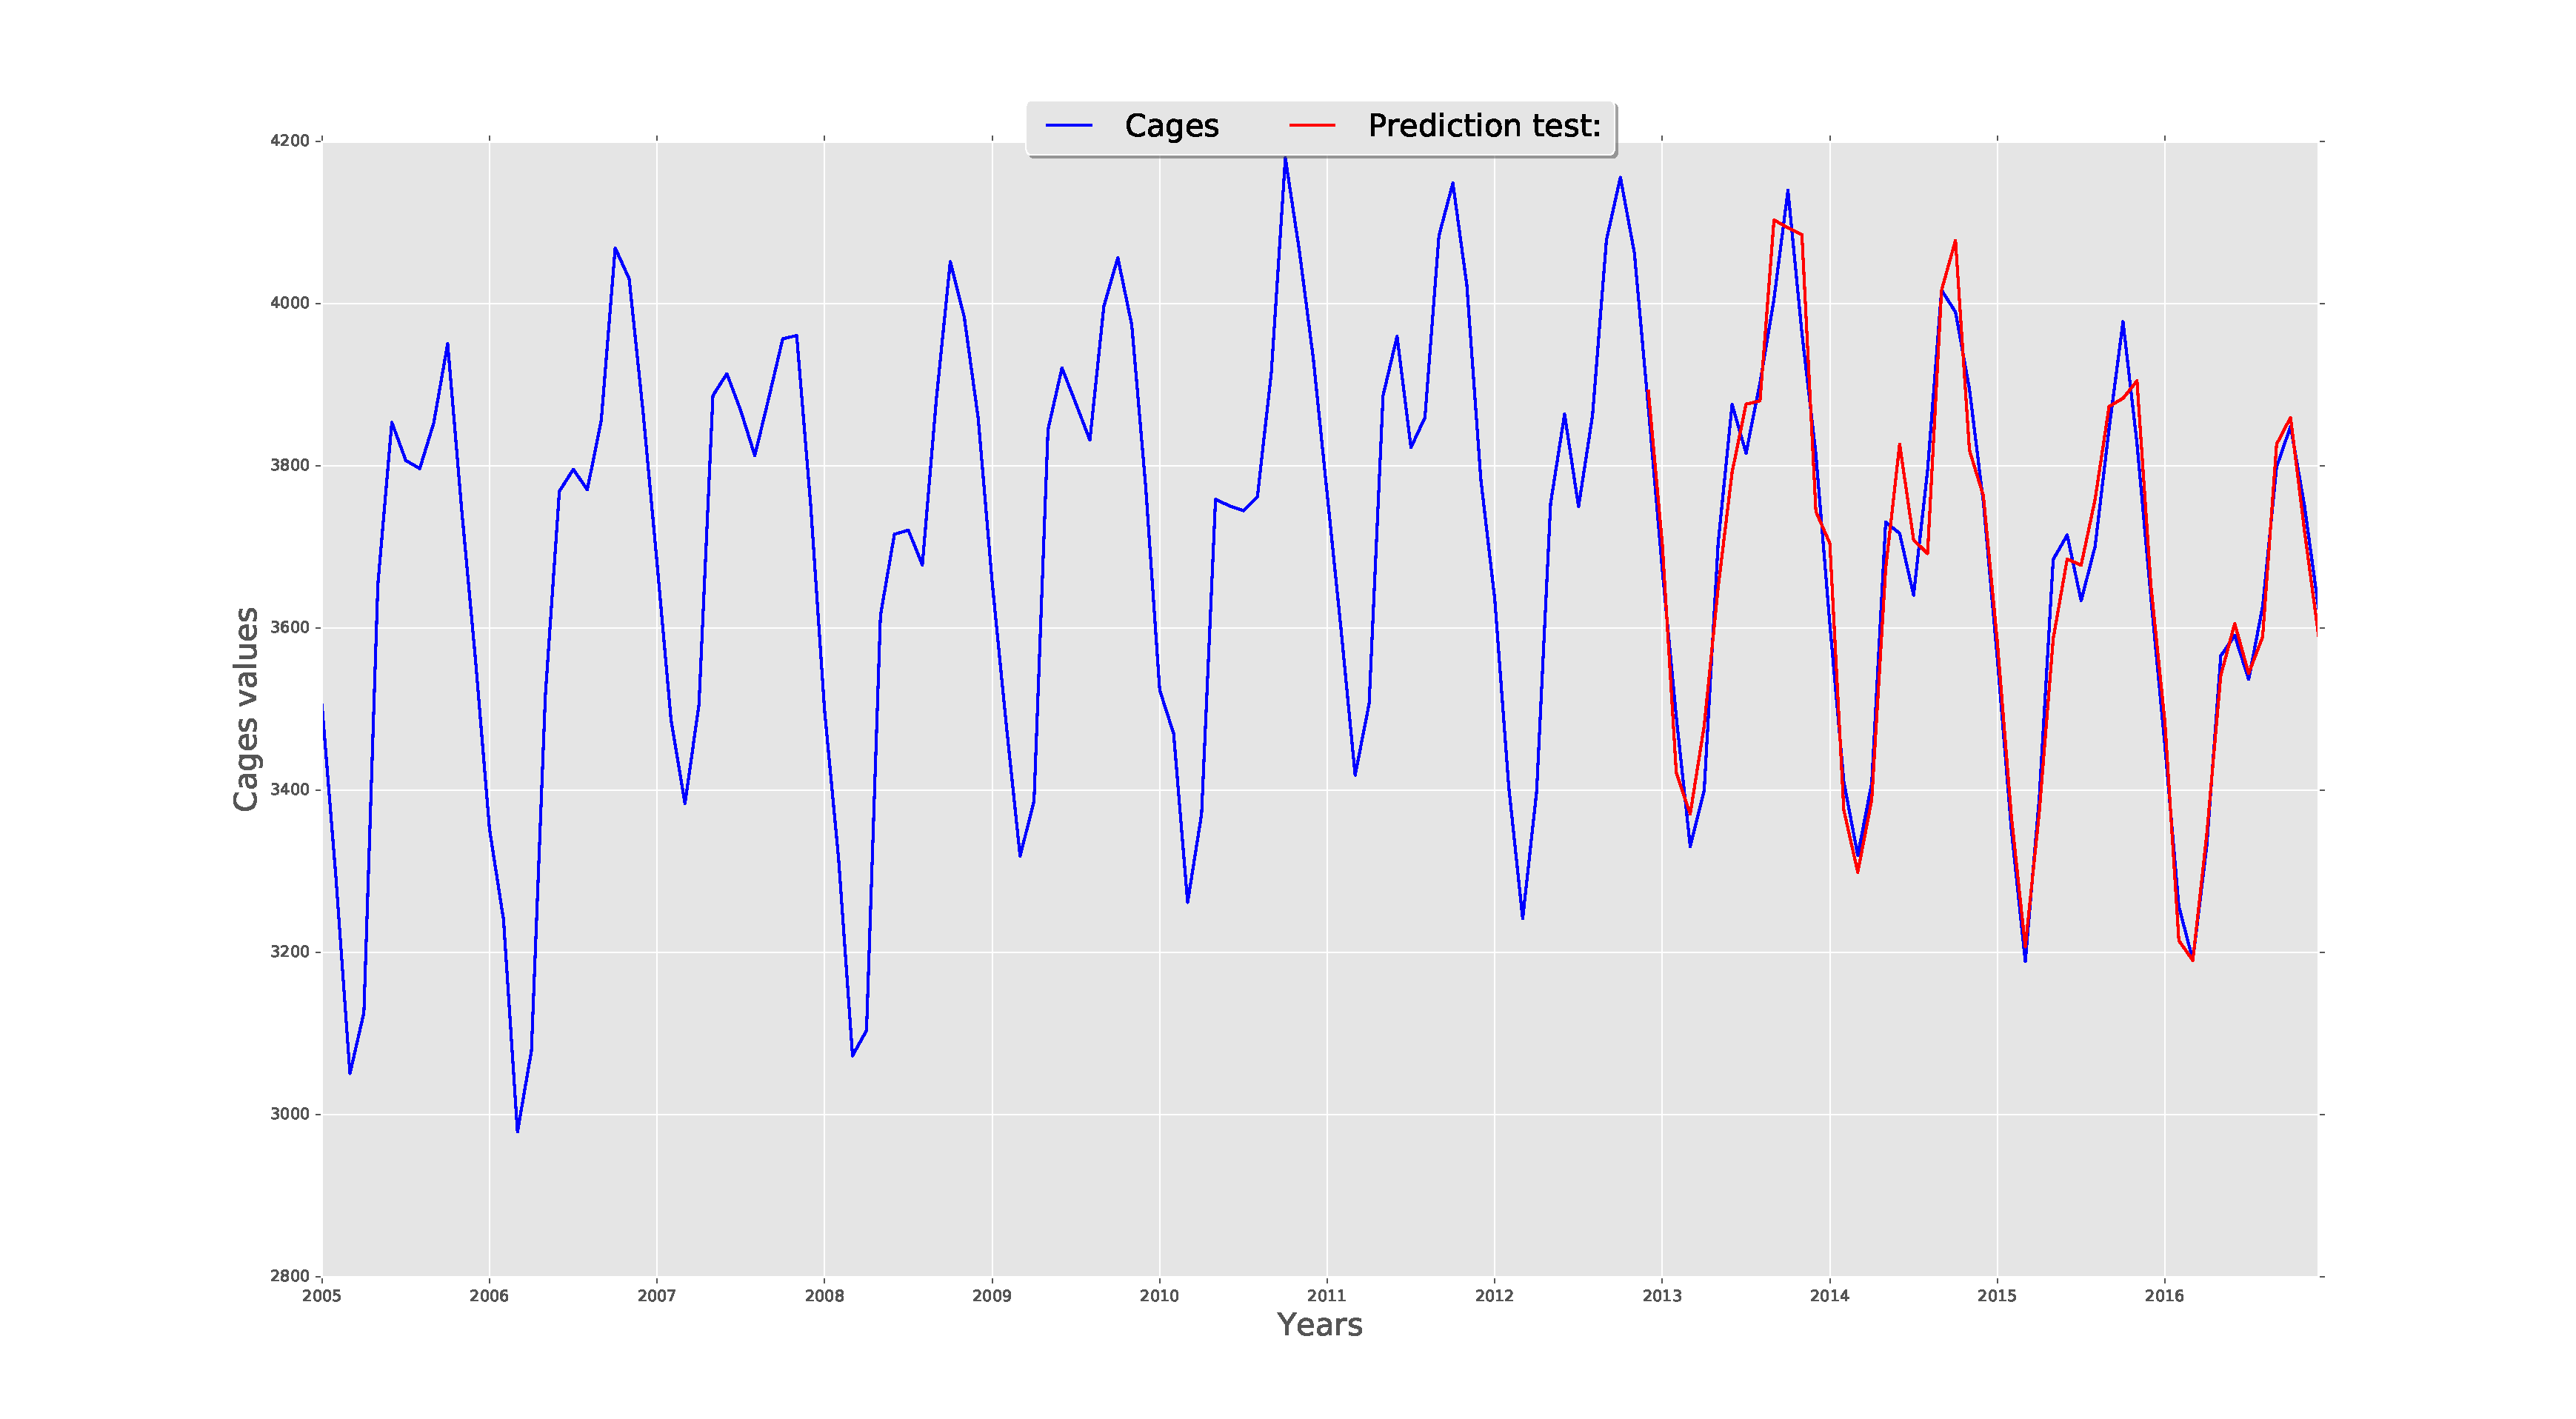
\includegraphics[width=1.5\textwidth]{Files/Cages_TRAIN.pdf}}
    \caption{Graphic that displays the predicted values from a particular ARIMA machine configuration and the historic real values.}
\end{figure}


\newpage
\subsection{Future Prediction System}
\textbf{Goal:}\\ 
This part of the work has the goal of display some real prediction of values in the future. \\
It basically collects real future values, in this particular are values about 2017, of each single input and then, once calculated also the prediction values, it's going to display on the same graphic:\\
- Historic values\\
- Predicted future values\\
- Real values (if are available)

\textbf{Requirements:}\\
This system has to be as much reusable as possible, so there are not that strict requirements. You can reuse this Future Prediction System with any kind of dataset with no restrictions about length. \\
The only requirement to let it works in a proper way is that you have to set the historic and real values datasets in the right way; it means that you have to write down the historic values in the dataset in this way:


\begin{table}[ht] 
    \centering 
    \begin{tabular}{ | l | l | l | p{5cm} |}
        \hline
        Index 	& Input1 	& Input2			\\ \hline
          	1 	& Value1 	& Value1			\\ \hline
          	2 	& Value2 	& Value2			\\ \hline
          	3 	& Value3	& Value3 		\\ \hline
          	... & ... 		& ...				\\ \hline
           	120 & Value120 & Value120	\\ \hline
          	121 & Value121 & Value121	\\ \hline
 			122 & Value122 & Value122	\\ \hline
    \end{tabular}
    \caption{Historic dataset structure}
    \label{table: pred_historic_values} 
\end{table} 

And then, if you want to compare the predicted values with some real values that are already available, you have to set the real values dataset in this way:


\begin{table}[ht] 
    \centering 
    \begin{tabular}{ | l | l | l | p{5cm} |}
        \hline
        Index & Input1 & Input2 		\\ \hline
          	123 & Value123 & Value123 	\\ \hline
          	124 & Value124 & Value124 	\\ \hline
          	125 & Value125 & Value125 	\\ \hline
          	126 & 	&					\\ \hline
          	127 & 	&					\\ \hline
          	128 & 	&					\\ \hline
 			129 & 	&					\\ \hline
    \end{tabular}
    \caption{Future real values dataset structure}
    \label{table: pred_real_values} 
\end{table} 

\newpage

\textbf{Code implementation:}\\
\begin{lstlisting}
model = ARIMA(history, order=arima_order)
model_fit = model.fit(disp=0)
yhat = model_fit.forecast()[0]
\end{lstlisting}


\begin{lstlisting}
# 1) Historic values
series = pd.read_csv("HISTORIC DATASET", 
			usecols=[sys.argv[1]])
series.plot(color="blue",linewidth=1.5)

# 2) Predicted future values
series = Series.from_csv("PREDICTIONS DATASET")
series.plot(color="red", linewidth=1.5, 
			label="Prediction Results")

# 3) Real future values
series = pd.read_csv("REAL VALUES DATASET")
pyplot.plot(series["Index"], series[sys.argv[1]],
	color="green", linewidth=1.5, label="Real values")

\end{lstlisting}
\textbf{Results:}\\
The system implemented during this phase allows to predict future for as many months as you want in the future and to display it, compared also with the historic values and real values once are available.
\begin{figure}[H]
	\centering
    \makebox[\textwidth][c]{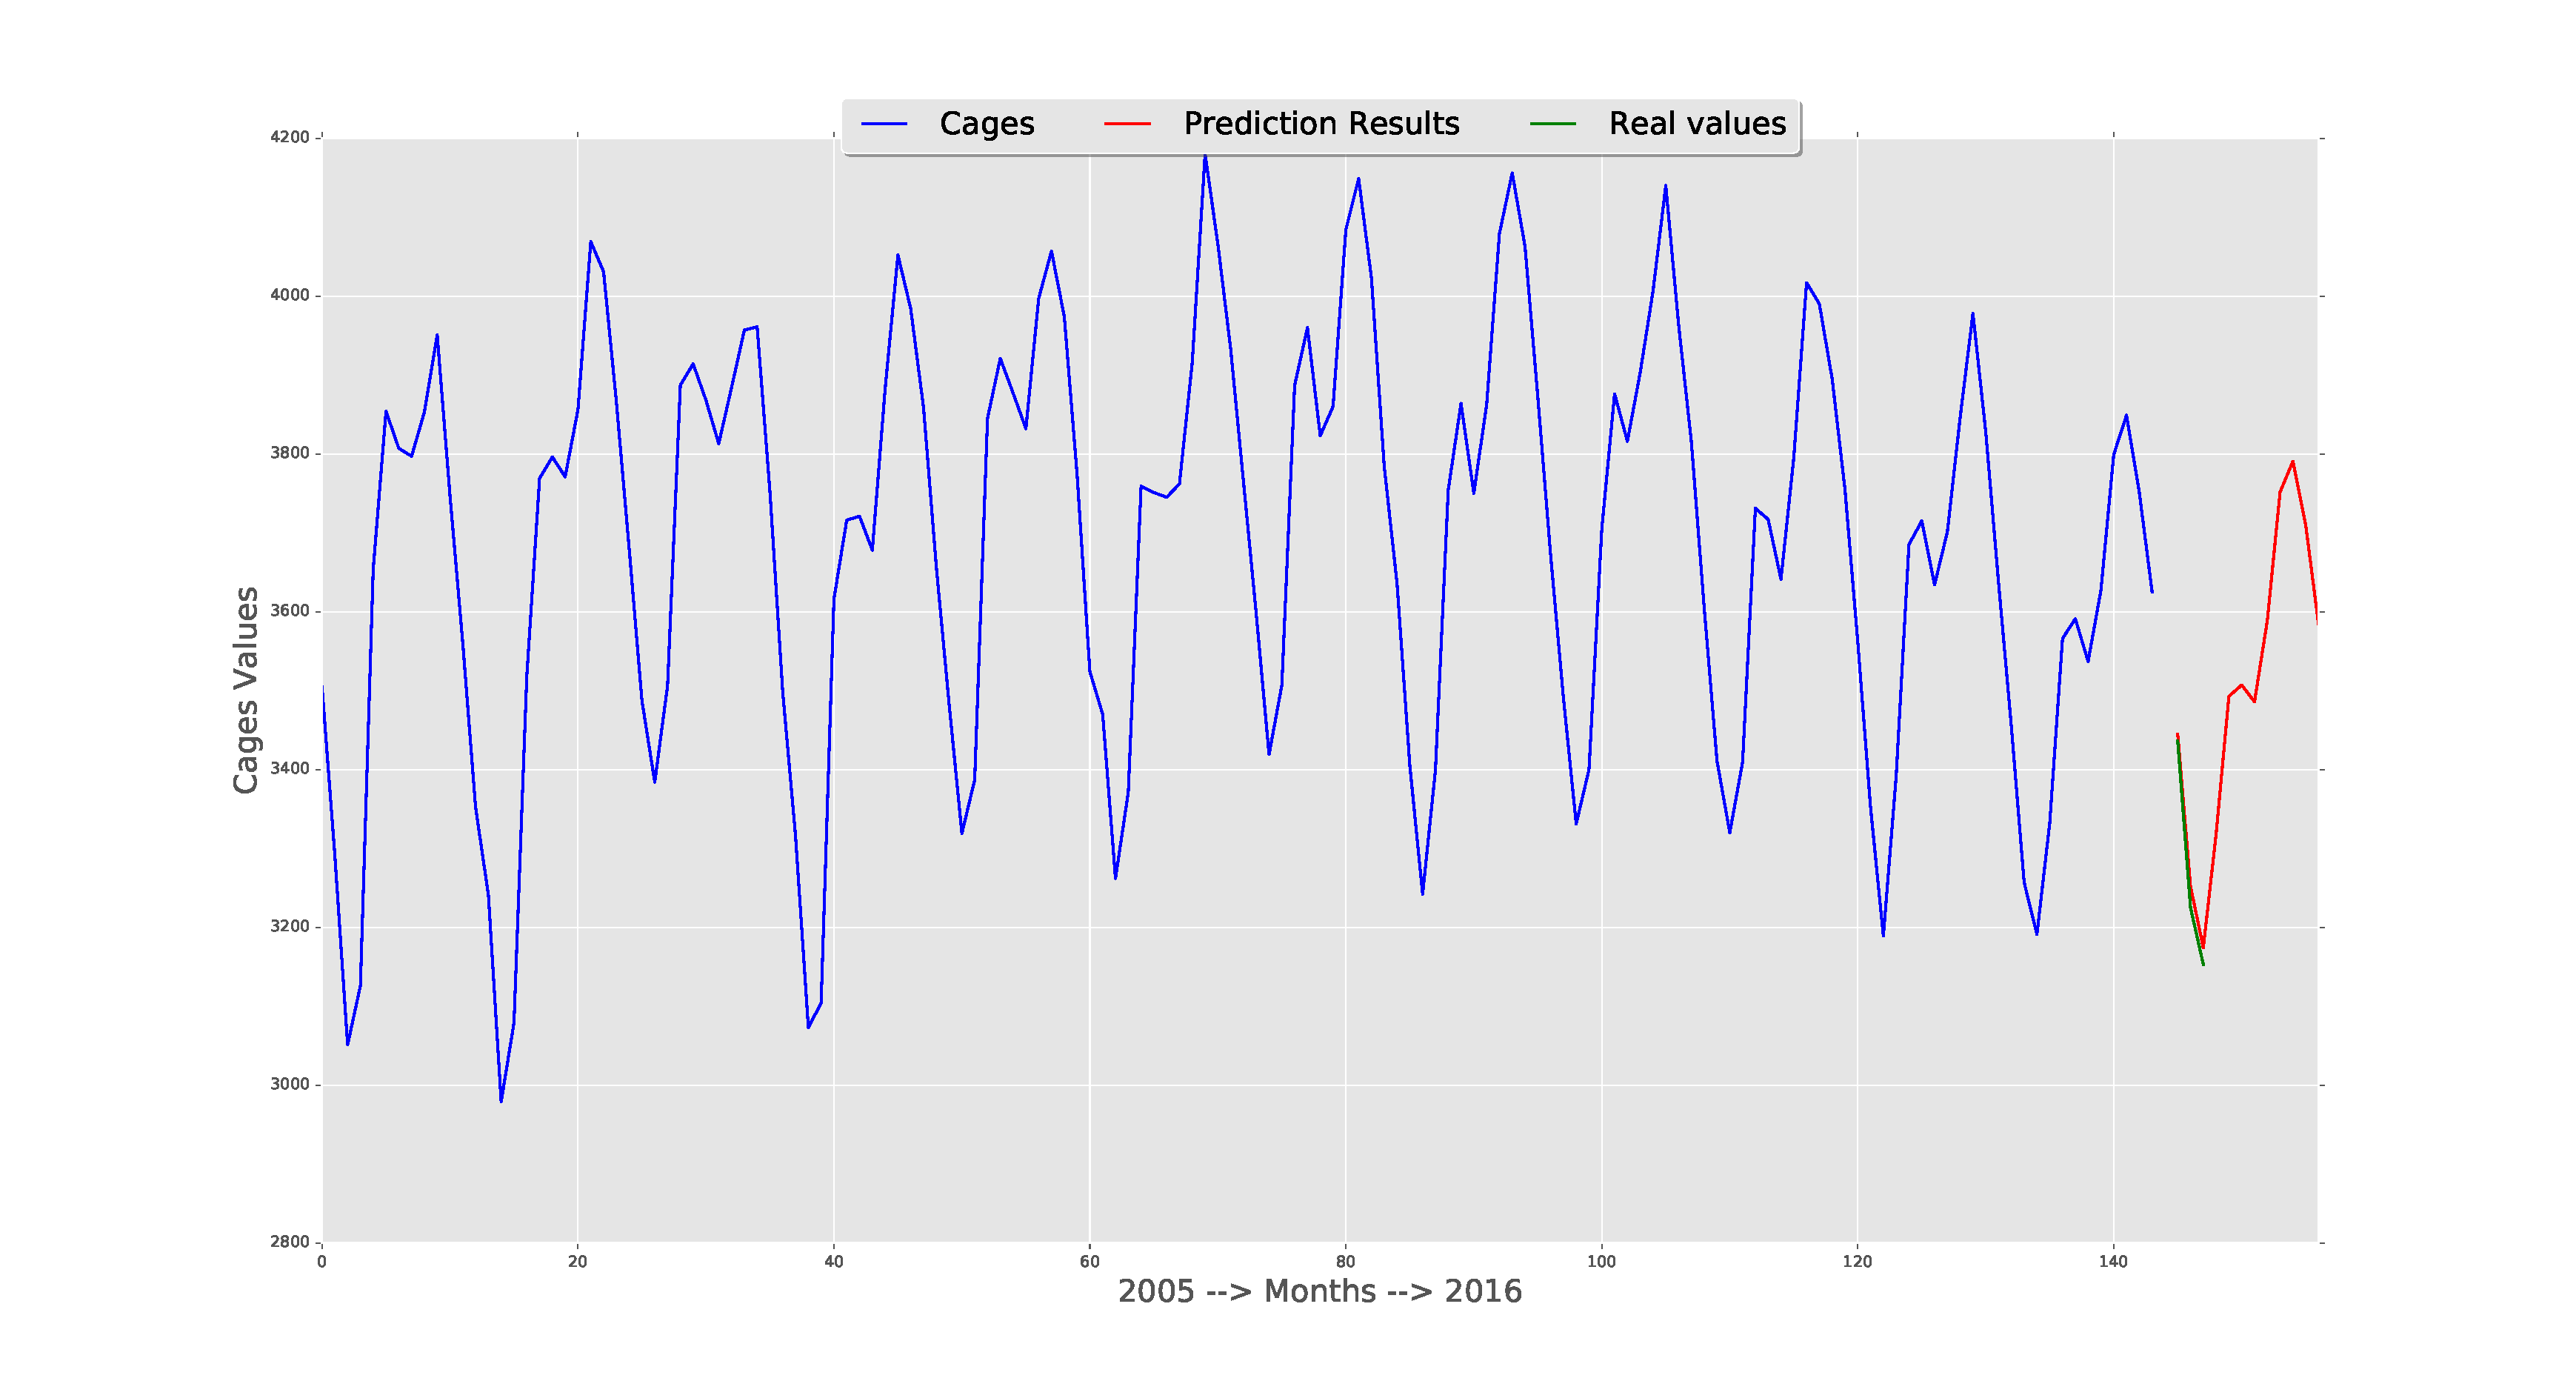
\includegraphics[width=1.5\textwidth]{Files/Cages_Predictions.pdf}}
    \caption{Graphic that display historic, future and predicted values of a input.}
\end{figure}

\newpage

\section{Requirements for reusability}
The subsystems implemented during this phase of the work are almost completely reusable.\\
The reusability this systems allows to get some prediction of values about different kind of dataset, in particular:
\begin{itemize}
\item The "Evaluating System" is actually 100\% reusable, and you can use it for evaluate any kind of dataset.
\item The "Future Prediction System" is completely reusable as well, you should only modify the historic values and the real values inside the dataset for it works in a proper way.
\item The "Training System" has been implemented for testing the current dataset, so it's not completely reusable but could be changed very easily and let it works also for other data input.
\end{itemize}


